\newcommand{\figureLCDChar}[1]{
  \def\lang{\detokenize{#1}}
  \def\langRu{\detokenize{ru}}
  \def\langEn{\detokenize{en}}
  \def\figureCaption{XXX: No translation.}
  \ifx \lang\langRu
  \def\figureCaption{
    Схематическое изображение клетки, в которой отрисовывается символ.
  }
  \fi
  \ifx \lang\langEn
  \def\figureCaption{
    A schematic representation of a cell on LCD screen where a character can be
    drawn.
  }
  \fi
  \begin{figure}[ht]
    \centering
    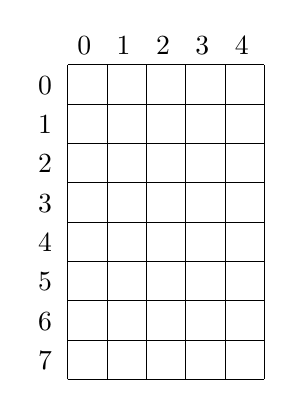
\begin{tikzpicture}
      \draw[step=0.5cm,black,very thin] (-2.5, -4) grid (0, 0);
      \foreach[count=\n from 0] \x in {-2.5, -2.0, ..., -0.5} {
        \draw (\x cm, 0) node[anchor=south west] {$\n$};
      }
      \foreach[count=\n from 0] \y in {-0.5, -1.0, ..., -4} {
        \draw (-3.0, \y) node[anchor=south west] {$\n$};
      }
    \end{tikzpicture}
    \caption{\figureCaption}
    \label{fig:game-dev-char}
  \end{figure}
}
